\documentclass[10pt]{article}
\usepackage[letterpaper,margin=0.72in,headheight=15pt]{geometry}
\usepackage[T1]{fontenc}
\usepackage[utf8]{inputenc}
\usepackage{lmodern}
\usepackage{microtype}
\usepackage{parskip}
\usepackage{enumitem}
\usepackage{booktabs}
\usepackage{tabularx}
\usepackage{longtable}
\usepackage{array}
\usepackage{xcolor}
\usepackage[most]{tcolorbox}
\usepackage{fancyhdr}
\usepackage{hyperref}
\usepackage{amsmath,amssymb}
\usepackage{listings}
\usepackage{tikz}
\usetikzlibrary{arrows.meta,positioning,shapes.geometric,fit}
\usepackage{needspace}
\usepackage{multicol}
\usepackage{lastpage}
\usepackage{titlesec}

\definecolor{navy}{HTML}{17324D}
\definecolor{bluegray}{HTML}{43657D}
\definecolor{lightblue}{HTML}{EAF2F8}
\definecolor{lightgray}{HTML}{F3F5F7}
\definecolor{linegray}{HTML}{C9D1D9}
\definecolor{darkgray}{HTML}{4A5561}
\definecolor{accent}{HTML}{8E3B46}

\hypersetup{colorlinks=true,linkcolor=navy,urlcolor=bluegray,citecolor=navy,pdfborder={0 0 0}}
\setlist[itemize]{leftmargin=1.4em,itemsep=2pt,topsep=4pt}
\setlist[enumerate]{leftmargin=1.6em,itemsep=2pt,topsep=4pt}
\renewcommand{\arraystretch}{1.22}
\setlength{\tabcolsep}{4pt}
\newcolumntype{Y}{>{\raggedright\arraybackslash}X}
\newcolumntype{C}[1]{>{\centering\arraybackslash}p{#1}}
\newcolumntype{L}[1]{>{\raggedright\arraybackslash}p{#1}}
\pagestyle{fancy}
\fancyhf{}
\lhead{Application Security Engineering}
\rhead{Code Review Handbook}
\cfoot{\thepage\ of \pageref{LastPage}}
\renewcommand{\headrulewidth}{0.4pt}
\titleformat{\section}{\Large\bfseries\color{navy}}{\thesection}{0.65em}{}
\titleformat{\subsection}{\large\bfseries\color{bluegray}}{\thesubsection}{0.55em}{}
\titleformat{\subsubsection}{\normalsize\bfseries\color{darkgray}}{\thesubsubsection}{0.5em}{}
\titlespacing*{\section}{0pt}{1.4em}{0.55em}
\titlespacing*{\subsection}{0pt}{1.0em}{0.35em}

\newcommand{\checkbox}{\ensuremath{\square}}
\newcommand{\fieldline}[1]{\textbf{#1}\hspace{0.5em}\leaders\hbox{\rule[0.4ex]{0.6em}{0.35pt}\hspace{0.25em}}\hfill\kern0pt}
\newcommand{\workarea}[1]{\par\smallskip\noindent\begin{tcolorbox}[height=#1,colback=white,colframe=linegray,boxrule=0.5pt,arc=0pt,left=2pt,right=2pt,top=2pt,bottom=2pt]\mbox{}\end{tcolorbox}\par}
\newtcolorbox{keybox}[1]{colback=lightblue,colframe=bluegray,title=\textbf{#1},fonttitle=\bfseries,boxrule=0.7pt,arc=2pt,left=6pt,right=6pt,top=5pt,bottom=5pt}
\newtcolorbox{cautionbox}[1]{colback=lightgray,colframe=accent,title=\textbf{#1},fonttitle=\bfseries,boxrule=0.7pt,arc=2pt,left=6pt,right=6pt,top=5pt,bottom=5pt}
\newtcolorbox{worksheetbox}[1]{colback=white,colframe=linegray,title=\textbf{#1},fonttitle=\bfseries,coltitle=navy,boxrule=0.6pt,arc=1pt,left=6pt,right=6pt,top=5pt,bottom=5pt}
\lstset{basicstyle=\ttfamily\small,columns=fullflexible,breaklines=true,frame=single,framerule=0.4pt,rulecolor=\color{linegray},backgroundcolor=\color{lightgray},showstringspaces=false,tabsize=2,keywordstyle=\bfseries}
\setcounter{tocdepth}{2}

\title{\textbf{Code Audit Techniques Catalog}\\\large Application Security Engineering Handout}
\author{}
\date{}

\begin{document}
\maketitle
\thispagestyle{empty}
\begin{keybox}{Purpose}
Practitioner catalog of localized analysis techniques used while executing code-audit strategies.
\end{keybox}
\vfill
\noindent\textbf{Use note.} This handout is a practitioner aid for authorized software security assessment. It emphasizes evidence, traceability, and disciplined review rather than a single rigid methodology.
\newpage
\tableofcontents
\newpage

\section{Catalog Use}
A \textbf{strategy} determines the route through the assessment. A \textbf{technique} is a local method applied while executing that route. For example, a reviewer may choose the ``Analyze an Algorithm'' strategy, then use internal flow analysis, desk-checking, and targeted test cases inside that algorithm.

\begin{center}
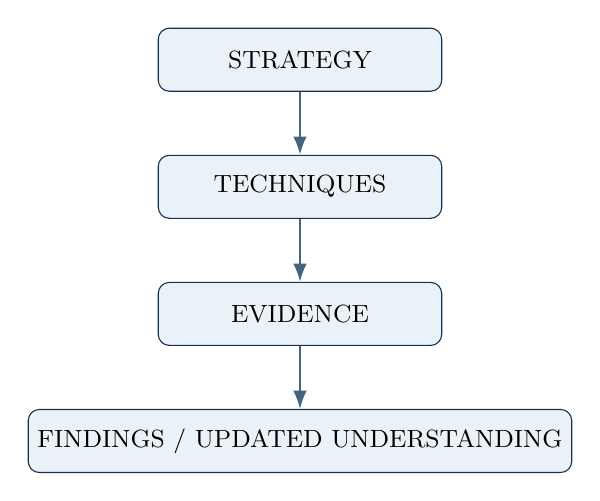
\begin{tikzpicture}[node distance=8mm, box/.style={draw=navy,rounded corners,minimum width=3.6cm,minimum height=.8cm,align=center,fill=lightblue,font=\small}, arr/.style={-Latex,thick,color=bluegray}]
\node[box] (s) {STRATEGY};
\node[box,below=of s] (t) {TECHNIQUES};
\node[box,below=of t] (e) {EVIDENCE};
\node[box,below=of e] (f) {FINDINGS / UPDATED UNDERSTANDING};
\draw[arr] (s)--(t);\draw[arr] (t)--(e);\draw[arr] (e)--(f);
\end{tikzpicture}
\end{center}

\section{Technique Selection Guide}
\par\smallskip\noindent\begin{tabularx}{\linewidth}{@{}L{0.28\linewidth}Y@{}}
\toprule
Observed review problem & Technique to consider \\
\midrule
Branch-heavy or confusing local control flow & Internal Flow Analysis; Desk-Checking \\
Custom wrappers or hidden shared behavior & Subsystem and Dependency Analysis \\
Reviewer may be overlooking a concern class & Rereading / Multi-Pass Review \\
Exact boundary/state values are hard to reason about & Desk-Checking; Test Case Construction \\
Large input combination space & Constraint Establishment; Extraneous Input Thinning \\
Code trusts upstream validation & Hostile-Input Assumption \\
Strings / encoded / structured data & Unconstrained Data Analysis \\
Critical reasoning remains uncertain & Peer Review of Complex Analysis \\
\bottomrule
\end{tabularx}

\Needspace{16\baselineskip}
\section{Technique 1 -- Internal Flow Analysis}
\par\smallskip\noindent\begin{tabularx}{\linewidth}{@{}L{0.24\linewidth}Y@{}}
\toprule
Purpose & Reason precisely about intraprocedural control flow and data flow. \\
Problem it solves & Complex branching, error handling, and local state interactions can hide paths that a linear read misses. \\
When to use & When a function or code fragment has meaningful branches, loops, early returns, side effects, or security-sensitive local state. \\
Inputs required & Selected function, local variables/state, known input constraints, intended postconditions. \\
Evidence produced & Path notes, branch matrix, state transitions, candidate findings. \\
Common mistakes & Treating error paths as inherently uninteresting; assuming logical impossibility without proving implementation constraints. \\
Limitations & Path count can grow rapidly; analysis is local unless paired with external tracing. \\
Works well with & Desk-checking, rereading, test cases, peer review \\
Example & A validation failure returns before a lock is released, leaving a resource held. \\
Reviewer completion test & Confirm each security-relevant exit, branch, and state transition has been considered. \\
\bottomrule
\end{tabularx}
\subsection*{Step-by-Step Procedure}
\begin{enumerate}
\item Enumerate normal, error, and exceptional exits.
\item Identify branch conditions and state mutations.
\item Trace relevant local data through assignments and calls.
\item Examine error-checking branches even when they appear unlikely.
\item Isolate pathological combinations in branch-heavy functions.
\item Record security-relevant paths, unreachable claims, and unresolved conditions.
\end{enumerate}
\subsection*{Security Questions}
\begin{itemize}
\item Which paths receive little normal testing?
\item Can a rare branch leave inconsistent state?
\item Can logically odd branch combinations occur because the implementation fails to forbid them?
\item Do early returns bypass cleanup, authorization, or state restoration?
\end{itemize}

\Needspace{16\baselineskip}
\section{Technique 2 -- Subsystem and Dependency Analysis}
\par\smallskip\noindent\begin{tabularx}{\linewidth}{@{}L{0.24\linewidth}Y@{}}
\toprule
Purpose & Understand shared subsystems whose behavior affects many reviewed paths. \\
Problem it solves & Security-relevant behavior can be hidden in wrappers, allocators, parsers, storage layers, or framework utilities that do not directly receive external input. \\
When to use & Early when custom shared infrastructure appears, and whenever a caller relies on unfamiliar dependency semantics. \\
Inputs required & Dependency inventory, wrappers/adapters, platform/API documentation available to the review. \\
Evidence produced & Dependency contract notes, wrapper differences, affected call sites, candidate patterns. \\
Common mistakes & Reviewing only entry-point modules; assuming familiar API names preserve platform semantics. \\
Limitations & May require platform knowledge and can become broad if dependency scope is not bounded. \\
Works well with & Module analysis, CP6, internal flow analysis \\
Example & A custom allocator rounds sizes differently than callers expect, invalidating length assumptions across multiple modules. \\
Reviewer completion test & Document every security-relevant semantic difference and the callers affected. \\
\bottomrule
\end{tabularx}
\subsection*{Step-by-Step Procedure}
\begin{enumerate}
\item Identify shared subsystems and custom wrappers.
\item State the behavior callers assume.
\item Inspect error contracts, ownership, sizing, normalization, and side effects.
\item Compare wrappers with underlying API semantics.
\item Trace how failures or surprising behavior propagate across callers/trust boundaries.
\item Promote recurring risky behavior into an application-specific candidate pattern.
\end{enumerate}
\subsection*{Security Questions}
\begin{itemize}
\item What invariant does this dependency establish?
\item What does it return on partial failure?
\item Does it silently transform data or units?
\item Can callers disagree about ownership, length, encoding, or error meaning?
\end{itemize}

\Needspace{16\baselineskip}
\section{Technique 3 -- Rereading / Multi-Pass Review}
\par\smallskip\noindent\begin{tabularx}{\linewidth}{@{}L{0.24\linewidth}Y@{}}
\toprule
Purpose & Reduce oversight by reviewing the same code under different concern sets. \\
Problem it solves & One pass encourages tunnel vision; subtle bugs appear when the reviewer changes the question being asked. \\
When to use & Complex or critical code, or any code where a single pass leaves uncertainty. \\
Inputs required & Selected code region plus a pass plan appropriate to its context. \\
Evidence produced & Pass tracker, changed assumptions, new candidates, validated understanding. \\
Common mistakes & Using a fixed pass checklist mechanically even when a concern is irrelevant; rereading without changing analytical focus. \\
Limitations & Costs time; the value decreases once the mental model and concern coverage stabilize. \\
Works well with & Internal flow, desk-checking, peer review \\
Example & After a logic pass, reread a parser focusing only on length arithmetic and then again on cleanup/error paths. \\
Reviewer completion test & At least two distinct perspectives for critical code, with context-appropriate additional passes. \\
\bottomrule
\end{tabularx}
\subsection*{Step-by-Step Procedure}
\begin{enumerate}
\item First pass: purpose, structure, and control flow.
\item Second pass: input/data flow and trust.
\item Additional passes as applicable: memory/resource management; arithmetic/type/boundaries; API contracts/return values; error handling; synchronization/state; policy enforcement.
\item Record issues by pass.
\item After context has improved, revisit the most critical code to verify the original mental model.
\end{enumerate}
\subsection*{Security Questions}
\begin{itemize}
\item What concern was intentionally ignored in the prior pass?
\item Did a later discovery change the interpretation of earlier code?
\item Are there global/member side effects or ignored return values?
\end{itemize}

\Needspace{16\baselineskip}
\section{Technique 4 -- Desk-Checking}
\par\smallskip\noindent\begin{tabularx}{\linewidth}{@{}L{0.24\linewidth}Y@{}}
\toprule
Purpose & Manually execute a difficult code fragment with chosen values and explicit state tracking. \\
Problem it solves & Mental simulation becomes unreliable when variables interact, assignments repeat, or side effects are non-obvious. \\
When to use & When boundary behavior, loops, state transitions, or variable relationships require exact step-by-step reasoning. \\
Inputs required & Bounded code fragment, initial values, relevant state fields, expected invariants. \\
Evidence produced & Execution table, triggering values, violated invariant, candidate finding. \\
Common mistakes & Skipping statements that seem obvious; failing to model external/shared state; not recording post-loop state. \\
Limitations & Manual and time-consuming; best for bounded code. \\
Works well with & Test cases, internal flow, variable relationships \\
Example & Step through a loop at the exact capacity boundary and discover that the terminator write occurs after the valid range. \\
Reviewer completion test & Another reviewer can reproduce the state table from the code and chosen inputs. \\
\bottomrule
\end{tabularx}
\subsection*{Step-by-Step Procedure}
\begin{enumerate}
\item Choose suspicious/boundary values.
\item Create state columns for variables and resources.
\item Execute each statement exactly.
\item Record branch outcomes and mutations.
\item Record post-loop and post-error-path state.
\item Compare final state with postconditions/invariants.
\end{enumerate}
\subsection*{Security Questions}
\begin{itemize}
\item What is the exact value after each transformation?
\item Which write/read occurs at the boundary?
\item What state persists after a failure?
\end{itemize}

\Needspace{16\baselineskip}
\section{Technique 5 -- Test Case Construction}
\par\smallskip\noindent\begin{tabularx}{\linewidth}{@{}L{0.24\linewidth}Y@{}}
\toprule
Purpose & Choose a compact set of inputs that exercises high-value boundaries and interactions. \\
Problem it solves & Exhaustive input enumeration is usually impossible; naive happy-path values miss implementation-created boundaries. \\
When to use & Whenever a function, algorithm, parser, or relationship can be reasoned about using representative states. \\
Inputs required & Input domains, implementation operations, relationships, constraints, attacker influence. \\
Evidence produced & Test matrix, relationship cases, discarded cases with rationale. \\
Common mistakes & Assuming type boundaries are sufficient; multiplying every input state without pruning; pruning based on intuition rather than proof. \\
Limitations & Coverage remains representative, not exhaustive. \\
Works well with & Desk-checking, constraint establishment, unconstrained data analysis \\
Example & Test count*element-size around the multiplication limit and then test the fixed-overhead addition boundary separately. \\
Reviewer completion test & Every selected case maps to a boundary, relationship, security invariant, or explicit hypothesis. \\
\bottomrule
\end{tabularx}
\subsection*{Step-by-Step Procedure}
\begin{enumerate}
\item Partition values into meaningful ranges/states.
\item Select boundary and near-boundary representatives.
\item Inspect code for artificial boundaries created by arithmetic, conversion, rounding, normalization, or indexing.
\item Identify relationships between multiple inputs and derived state.
\item Add combinations that stress those relationships.
\item Use constraint establishment and extraneous-input thinning only with evidence.
\end{enumerate}
\subsection*{Security Questions}
\begin{itemize}
\item Which boundaries come from the code rather than the type/domain?
\item Which variables gain meaning only relative to another variable?
\item Which cases differ just before/at/after a check?
\end{itemize}

\Needspace{16\baselineskip}
\section{Technique 6 -- Hostile-Input Assumption}
\par\smallskip\noindent\begin{tabularx}{\linewidth}{@{}L{0.24\linewidth}Y@{}}
\toprule
Purpose & Challenge trust placed in data arriving from other modules or earlier validation stages. \\
Problem it solves & Developers often assume internal data is safe because some prior path was expected to sanitize it. \\
When to use & At module boundaries, general-purpose libraries, shared helpers, and security-sensitive consumers. \\
Inputs required & Data source, callers, sanitization locations, alternate paths, future extensibility assumptions. \\
Evidence produced & Trust assumptions, validation evidence, bypass possibilities, recommended local invariant checks. \\
Common mistakes & Treating every internal value as equally hostile as raw network input; alternatively, trusting it unconditionally. \\
Limitations & Appropriate skepticism depends on architecture and caller guarantees. \\
Works well with & Constraint establishment, dependency analysis, test cases \\
Example & A helper assumes a length was validated by an API handler, but a background job calls it directly with different constraints. \\
Reviewer completion test & Every security-sensitive assumption about upstream validation is documented and supported. \\
\bottomrule
\end{tabularx}
\subsection*{Step-by-Step Procedure}
\begin{enumerate}
\item Identify the data origin and all known callers.
\item Locate claimed validation/sanitization.
\item Check for alternate or future paths that bypass it.
\item Verify validation correctness and ordering relative to transformation.
\item Determine the minimum local consistency checks appropriate to the consumer.
\end{enumerate}
\subsection*{Security Questions}
\begin{itemize}
\item Can another caller reach this function with weaker guarantees?
\item Can transformation after validation invalidate the guarantee?
\item Is the consumer relying on undocumented caller discipline?
\end{itemize}

\Needspace{16\baselineskip}
\section{Technique 7 -- Constraint Establishment}
\par\smallskip\noindent\begin{tabularx}{\linewidth}{@{}L{0.24\linewidth}Y@{}}
\toprule
Purpose & Prune impossible test states only after proving the enforcing constraint. \\
Problem it solves & Large test spaces contain states that may be unreachable under the actual implementation. \\
When to use & After candidate states are enumerated and the reviewer needs to reduce them without losing meaningful coverage. \\
Inputs required & Potential state set, callers, guards, sanitizers, configuration constraints. \\
Evidence produced & Reduced test space plus proof/rationale for every removed state. \\
Common mistakes & Using ``unlikely as equivalent to impossible; failing to test the constraining check. \\
Limitations & Constraints can change over time as callers and code evolve. \\
Works well with & Test case construction, hostile-input assumption \\
Example & A wrapper proves length is positive on the only reachable call path, allowing negative cases to be removed after the wrapper is separately validated. \\
Reviewer completion test & No state is removed without a concrete enforcement location and bypass analysis. \\
\bottomrule
\end{tabularx}
\subsection*{Step-by-Step Procedure}
\begin{enumerate}
\item Enumerate candidate states first.
\item Identify the code or configuration claimed to prohibit a state.
\item Test or inspect the enforcing constraint itself.
\item Look for alternate callers, races, state changes, or bypasses.
\item Discard only states proven unreachable.
\item Record why each state was discarded.
\end{enumerate}
\subsection*{Security Questions}
\begin{itemize}
\item Is the constraint on every path?
\item Can the checked value change before use?
\item Does a different caller provide weaker guarantees?
\end{itemize}
\clearpage

\section{Technique 8 -- Extraneous Input Thinning}
\par\smallskip\noindent\begin{tabularx}{\linewidth}{@{}L{0.24\linewidth}Y@{}}
\toprule
Purpose & Remove input dimensions that neither attackers influence nor materially alter security-sensitive processing. \\
Problem it solves & Combinatorial input spaces become unmanageable when irrelevant variables are treated as independent security dimensions. \\
When to use & After identifying multiple inputs and their relationships. \\
Inputs required & Input sources, attacker-control analysis, control/data-flow influence. \\
Evidence produced & Thinned input matrix and rationale. \\
Common mistakes & Dropping uncontrollable inputs that still alter processing; ignoring indirect influence. \\
Limitations & Requires accurate influence analysis and may need revision as system understanding changes. \\
Works well with & Test cases, internal flow, dependency analysis \\
Example & A server flag set only by administrator configuration is still retained if it selects a parser mode that changes handling of remote input. \\
Reviewer completion test & Removed inputs satisfy both non-influence and non-impact conditions. \\
\bottomrule
\end{tabularx}
\subsection*{Step-by-Step Procedure}
\begin{enumerate}
\item For each input, determine direct and indirect attacker influence.
\item Determine whether changes affect how attacker-controlled data is handled or change security-sensitive behavior.
\item Remove only when both conditions are negative.
\item Retain output-only parameters or state as needed for execution reasoning even if initial value is irrelevant.
\item Document the rationale.
\end{enumerate}
\subsection*{Security Questions}
\begin{itemize}
\item Can the attacker influence configuration that sets this value?
\item Does this variable select a code path that changes validation or resource use?
\end{itemize}

\clearpage
\section{Technique 9 -- Unconstrained Data Analysis}
\par\smallskip\noindent\begin{tabularx}{\linewidth}{@{}L{0.24\linewidth}Y@{}}
\toprule
Purpose & Analyze strings and broad structured inputs by lifecycle operations rather than attempting exhaustive values. \\
Problem it solves & Arbitrary-length and structured data cannot be covered by a small numeric range. \\
When to use & Strings, encoded input, serialized data, document formats, protocol fields, and similar broad domains. \\
Inputs required & Data lifecycle from receipt through transformation, validation, parsing/extraction, and eventual system/resource use. \\
Evidence produced & Data-lifecycle map, stage-specific test cases, ordering hypotheses, final resource-use analysis. \\
Common mistakes & Validating one representation and using another; treating ``string as one undifferentiated input class. \\
Limitations & Requires knowledge of encodings, parser semantics, and downstream consumers. \\
Works well with & Test cases, hostile-input assumption, desk-checking \\
Example & Validate an encoded path before decoding, then show that decoding creates traversal syntax not present during validation. \\
Reviewer completion test & Every transformation, validation, parsing stage, and final resource use is accounted for. \\
\bottomrule
\end{tabularx}
\subsection*{Step-by-Step Procedure}
\begin{enumerate}
\item Map every transformation.
\item Map validations and state what later use they are supposed to make safe.
\item Map parsing/extraction boundaries and length sources.
\item Identify final system/resource uses.
\item Create boundary cases for each stage and especially for stage ordering.
\item Check whether one stage changes the representation assumed safe by an earlier stage.
\end{enumerate}
\subsection*{Security Questions}
\begin{itemize}
\item Does canonicalization happen before or after validation?
\item Can parsers disagree on delimiters or lengths?
\item Can transformed data select a different resource or namespace?
\end{itemize}

\clearpage
\section{Technique 10 -- Peer Review of Complex Analysis}
\par\smallskip\noindent\begin{tabularx}{\linewidth}{@{}L{0.24\linewidth}Y@{}}
\toprule
Purpose & Use an independent reviewer to challenge difficult reasoning or high-impact conclusions. \\
Problem it solves & Repeated exposure to the same code can solidify an incorrect mental model. \\
When to use & Complex algorithms, uncertain reasoning, critical trust boundaries, or major findings. \\
Inputs required & Code/evidence package and a clearly scoped question. \\
Evidence produced & Peer-review notes, resolved differences, added tests, confidence update. \\
Common mistakes & Turning peer review into a group discussion before independent reasoning; attempting to duplicate the entire audit. \\
Limitations & Expensive; should focus on high-value or uncertain areas. \\
Works well with & Hypothesis testing, desk-checking, design conformity \\
Example & Two reviewers independently analyze an authorization state machine, then compare allowed transitions and test the disputed edge cases. \\
Reviewer completion test & Material disagreements are resolved or explicitly recorded as residual uncertainty. \\
\bottomrule
\end{tabularx}
\subsection*{Step-by-Step Procedure}
\begin{enumerate}
\item Have the second reviewer analyze independently when practical.
\item Compare models, path assumptions, boundary cases, and finding rationale.
\item Resolve disagreements with code/runtime evidence.
\item Record remaining uncertainty.
\end{enumerate}
\subsection*{Security Questions}
\begin{itemize}
\item Did both reviewers infer the same contract and state transitions?
\item Which assumptions differ?
\item Can a disagreement be converted into a targeted test?
\end{itemize}

\section{Branch / Path Worksheet}
\begin{longtable}{@{}L{0.20\linewidth}L{0.18\linewidth}L{0.18\linewidth}L{0.17\linewidth}L{0.20\linewidth}@{}}
\toprule
Branch / condition & Input/state required & Resulting mutation & Error/cleanup effect & Security note \\
\midrule
\endfirsthead
\toprule
Branch / condition & Input/state required & Resulting mutation & Error/cleanup effect & Security note \\
\midrule
\endhead
\rule{0pt}{2.7em} & & & & \\
\rule{0pt}{2.7em} & & & & \\
\rule{0pt}{2.7em} & & & & \\
\rule{0pt}{2.7em} & & & & \\
\bottomrule
\end{longtable}

\section{Dependency Analysis Worksheet}
\begin{longtable}{@{}L{0.19\linewidth}L{0.20\linewidth}L{0.19\linewidth}L{0.17\linewidth}L{0.18\linewidth}@{}}
\toprule
Dependency & Caller assumption & Actual / observed behavior & Errors / side effects & Trust-boundary consequence \\
\midrule
\endfirsthead
\toprule
Dependency & Caller assumption & Actual / observed behavior & Errors / side effects & Trust-boundary consequence \\
\midrule
\endhead
Memory/resource management & & & & \\
Buffer abstraction & & & & \\
Parser / serializer & & & & \\
Filesystem wrapper & & & & \\
Network wrapper & & & & \\
Authentication helper & & & & \\
Authorization helper & & & & \\
Cryptographic wrapper & & & & \\
Framework utility & & & & \\
\bottomrule
\end{longtable}

\section{Multi-Pass Tracker}
\par\smallskip\noindent\begin{tabularx}{\linewidth}{@{}C{0.07\linewidth}L{0.29\linewidth}C{0.11\linewidth}Y@{}}
\toprule
Pass & Concern & Done? & New evidence / changed understanding \\
\midrule
1 & Purpose and control flow & & \\
2 & Input / data flow & & \\
3 & Memory / resource management & & \\
4 & Arithmetic / type / boundary behavior & & \\
5 & API contracts / return values & & \\
6 & Error handling & & \\
7 & State / synchronization & & \\
8 & Security-policy enforcement & & \\
\bottomrule
\end{tabularx}

\section{Data Lifecycle Worksheet}
\begin{longtable}{@{}C{0.06\linewidth}L{0.20\linewidth}L{0.19\linewidth}L{0.20\linewidth}L{0.28\linewidth}@{}}
\toprule
Step & Operation & Representation / state & Assumption established or consumed & Security question / test \\
\midrule
\endfirsthead
\toprule
Step & Operation & Representation / state & Assumption established or consumed & Security question / test \\
\midrule
\endhead
\rule{0pt}{2.7em} & & & & \\
\rule{0pt}{2.7em} & & & & \\
\rule{0pt}{2.7em} & & & & \\
\rule{0pt}{2.7em} & & & & \\
\rule{0pt}{2.7em} & & & & \\
\bottomrule
\end{longtable}
\clearpage

\section{Peer Review Checklist}
\begin{itemize}
\item[\checkbox] Scope and question are explicit.
\item[\checkbox] Reviewer can reproduce the path from supplied evidence.
\item[\checkbox] Assumptions and claimed constraints are listed separately from facts.
\item[\checkbox] Boundary values and state transitions were independently checked.
\item[\checkbox] Alternate callers / paths were considered.
\item[\checkbox] Security impact is separated from mere policy or specification deviation.
\item[\checkbox] Disagreements were resolved with code/runtime evidence or recorded as uncertainty.
\end{itemize}

\section{Compact Technique Checklist}
\begin{enumerate}
\item Analyze internal branches and error paths, not only the dominant happy path.
\item Learn the semantics of shared subsystems and wrappers before trusting caller assumptions.
\item Re-read critical code with a different concern set.
\item Desk-check exact values when mental simulation becomes unreliable.
\item Build test cases around both domain boundaries and boundaries created by implementation operations.
\item Treat upstream validation as an assumption to verify, not an axiom.
\item Establish constraints before pruning states; document every discarded case.
\item Thin only inputs that are both attacker-independent and behaviorally irrelevant to security-sensitive processing.
\item For unconstrained data, reason stage-by-stage through transformation, validation, parsing, and final system use.
\item Use independent peer review for the most complex, high-impact, or uncertain analysis.
\end{enumerate}
\end{document}
